% \addbibresource{refs.bib}

\section{Method} \label{section:method}
\subsection{Overview of an Image Retrieval System}

As described in Figure \ref{fig:image_retrieval_system}, a typical Image Retrieval System consists of 2 main steps: Feature Extraction and Similarity Matching. The Features Extraction step is explained in detail in section \ref{section:feature_extraction}. Subsequently, in section \ref{section:similarity_extraction}, the authors focus on describing how we perform Similarity Matching with our implementation of BoW model.


\subsection{Feature Extraction} \label{section:feature_extraction}

To detect and extract features from images, there are many methods that have been proposed (Harris-Affine, Hessian-Affine detectors \cite{Mikolajczyk2004}, Maximally stable extremal region (MSER) detector \cite{conf/bmvc/MatasCUP02}, Edge-based region detector \cite{Tuytelaars99content-basedimage}, Intensity extrema-based region detector \cite{Tuytelaars00widebaseline} ...). The authors choose to use Hessian-Affine detector, for detecting and extracting features from images. By using Hessian-Affine detector, which is also used in other baseline methods, our experiment's result can easily compare with other ones.

As we tested on Oxford Building 5K Dataset \cite{oxbuilding}, there are typically 3,300 features for each image and a total about 16 millions of features for the whole dataset. Then, we compute the SIFT descriptor \cite{Lowe2004} of all the features and these descriptors is used for matching images in the next step.

\begin{figure}
    \centering
    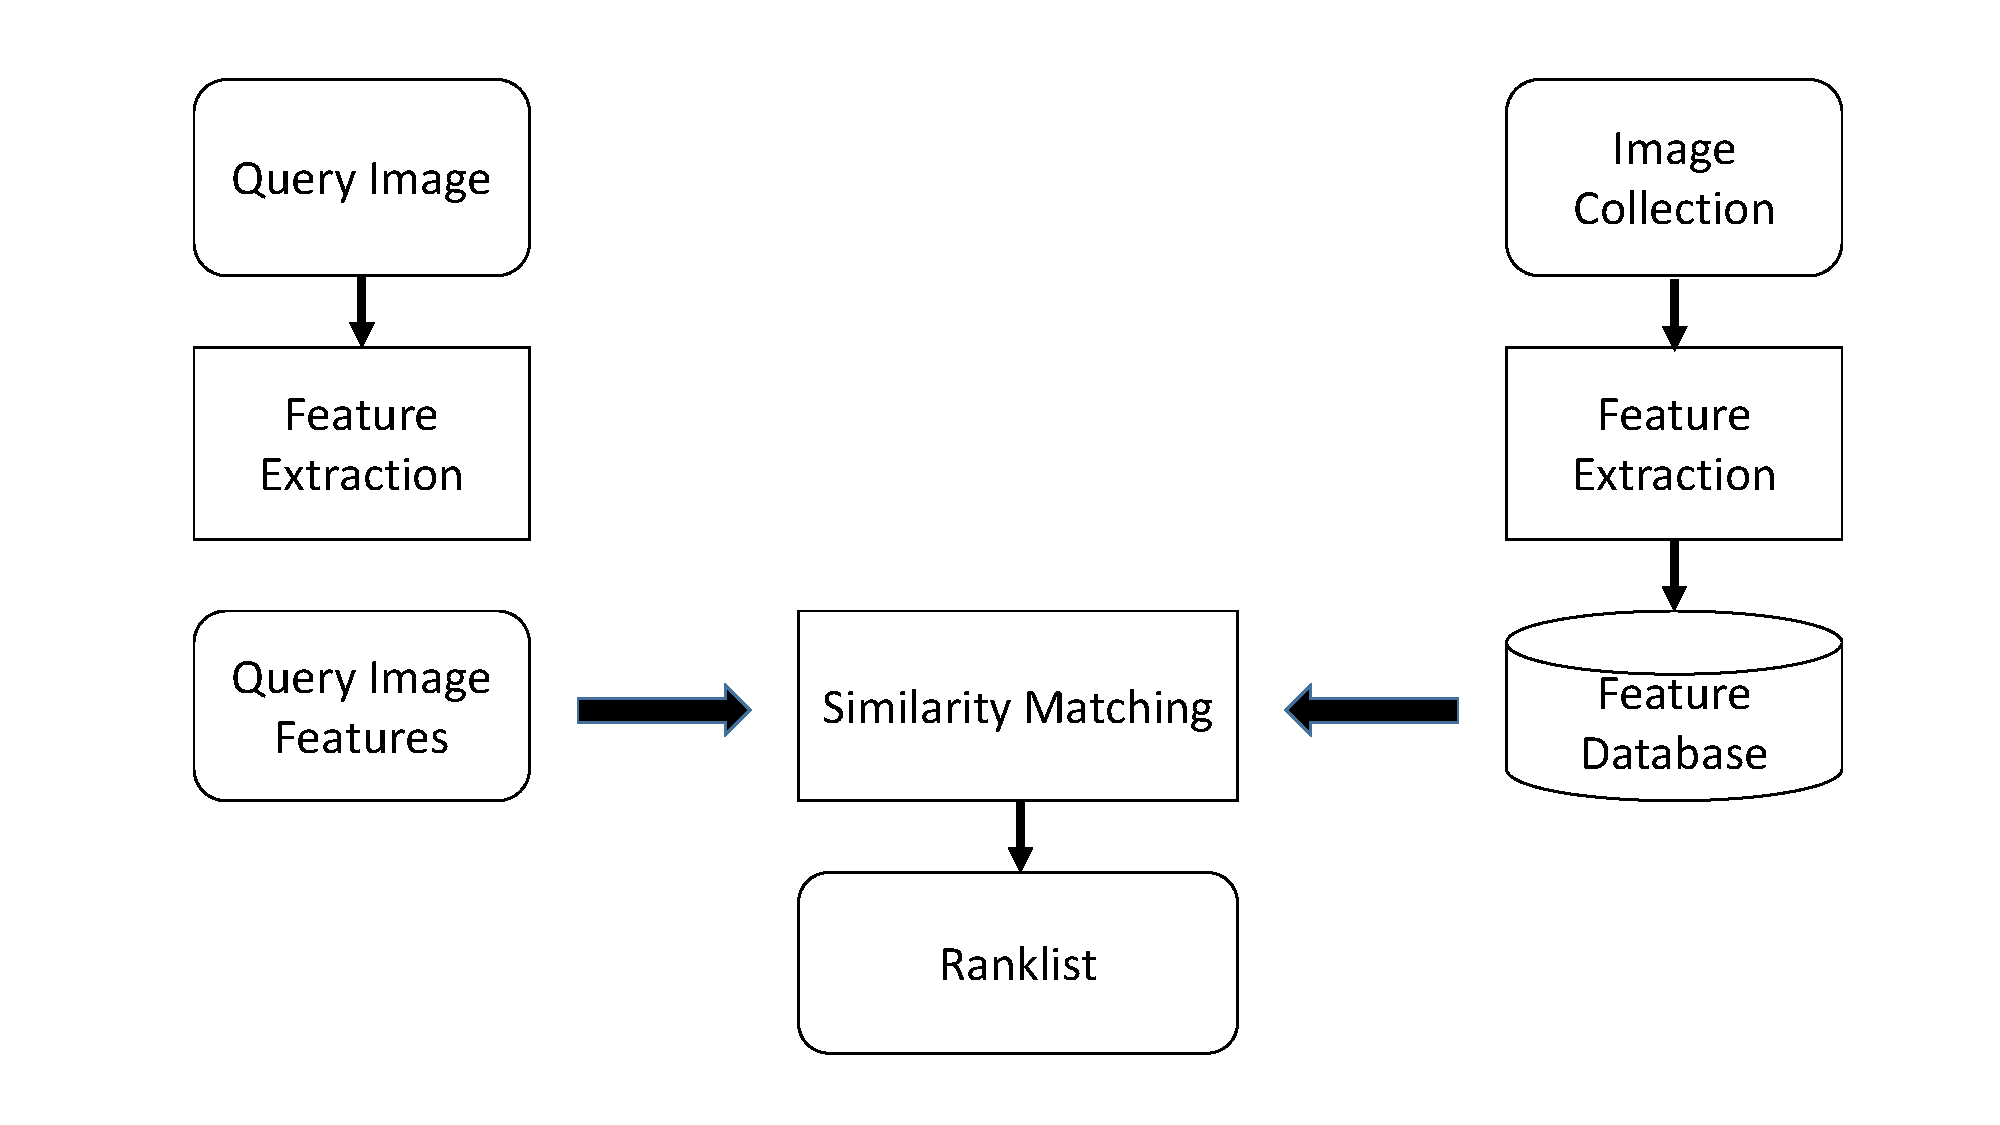
\includegraphics[width=3.0in]{ImageRetrievalSystem.pdf}
    \caption{How an image retrieval system works}
    \label{fig:image_retrieval_system}
\end{figure}

\subsection{Similarity Matching} \label{section:similarity_extraction}

As showed in Figure \ref{fig:bow_model} typical BoW model used in image retrieval systems would consist of the following steps: Dictionary Building, Quantization and Retrieving the result. The 2 former steps are described in section \ref{section:dictionary_building} and section \ref{section:quantization}. The last step is our main focus in this paper and is discussed in section \ref{section:tfidf_weighting} and section \ref{section:spatial_rerank}.

\begin{figure}
    \centering
    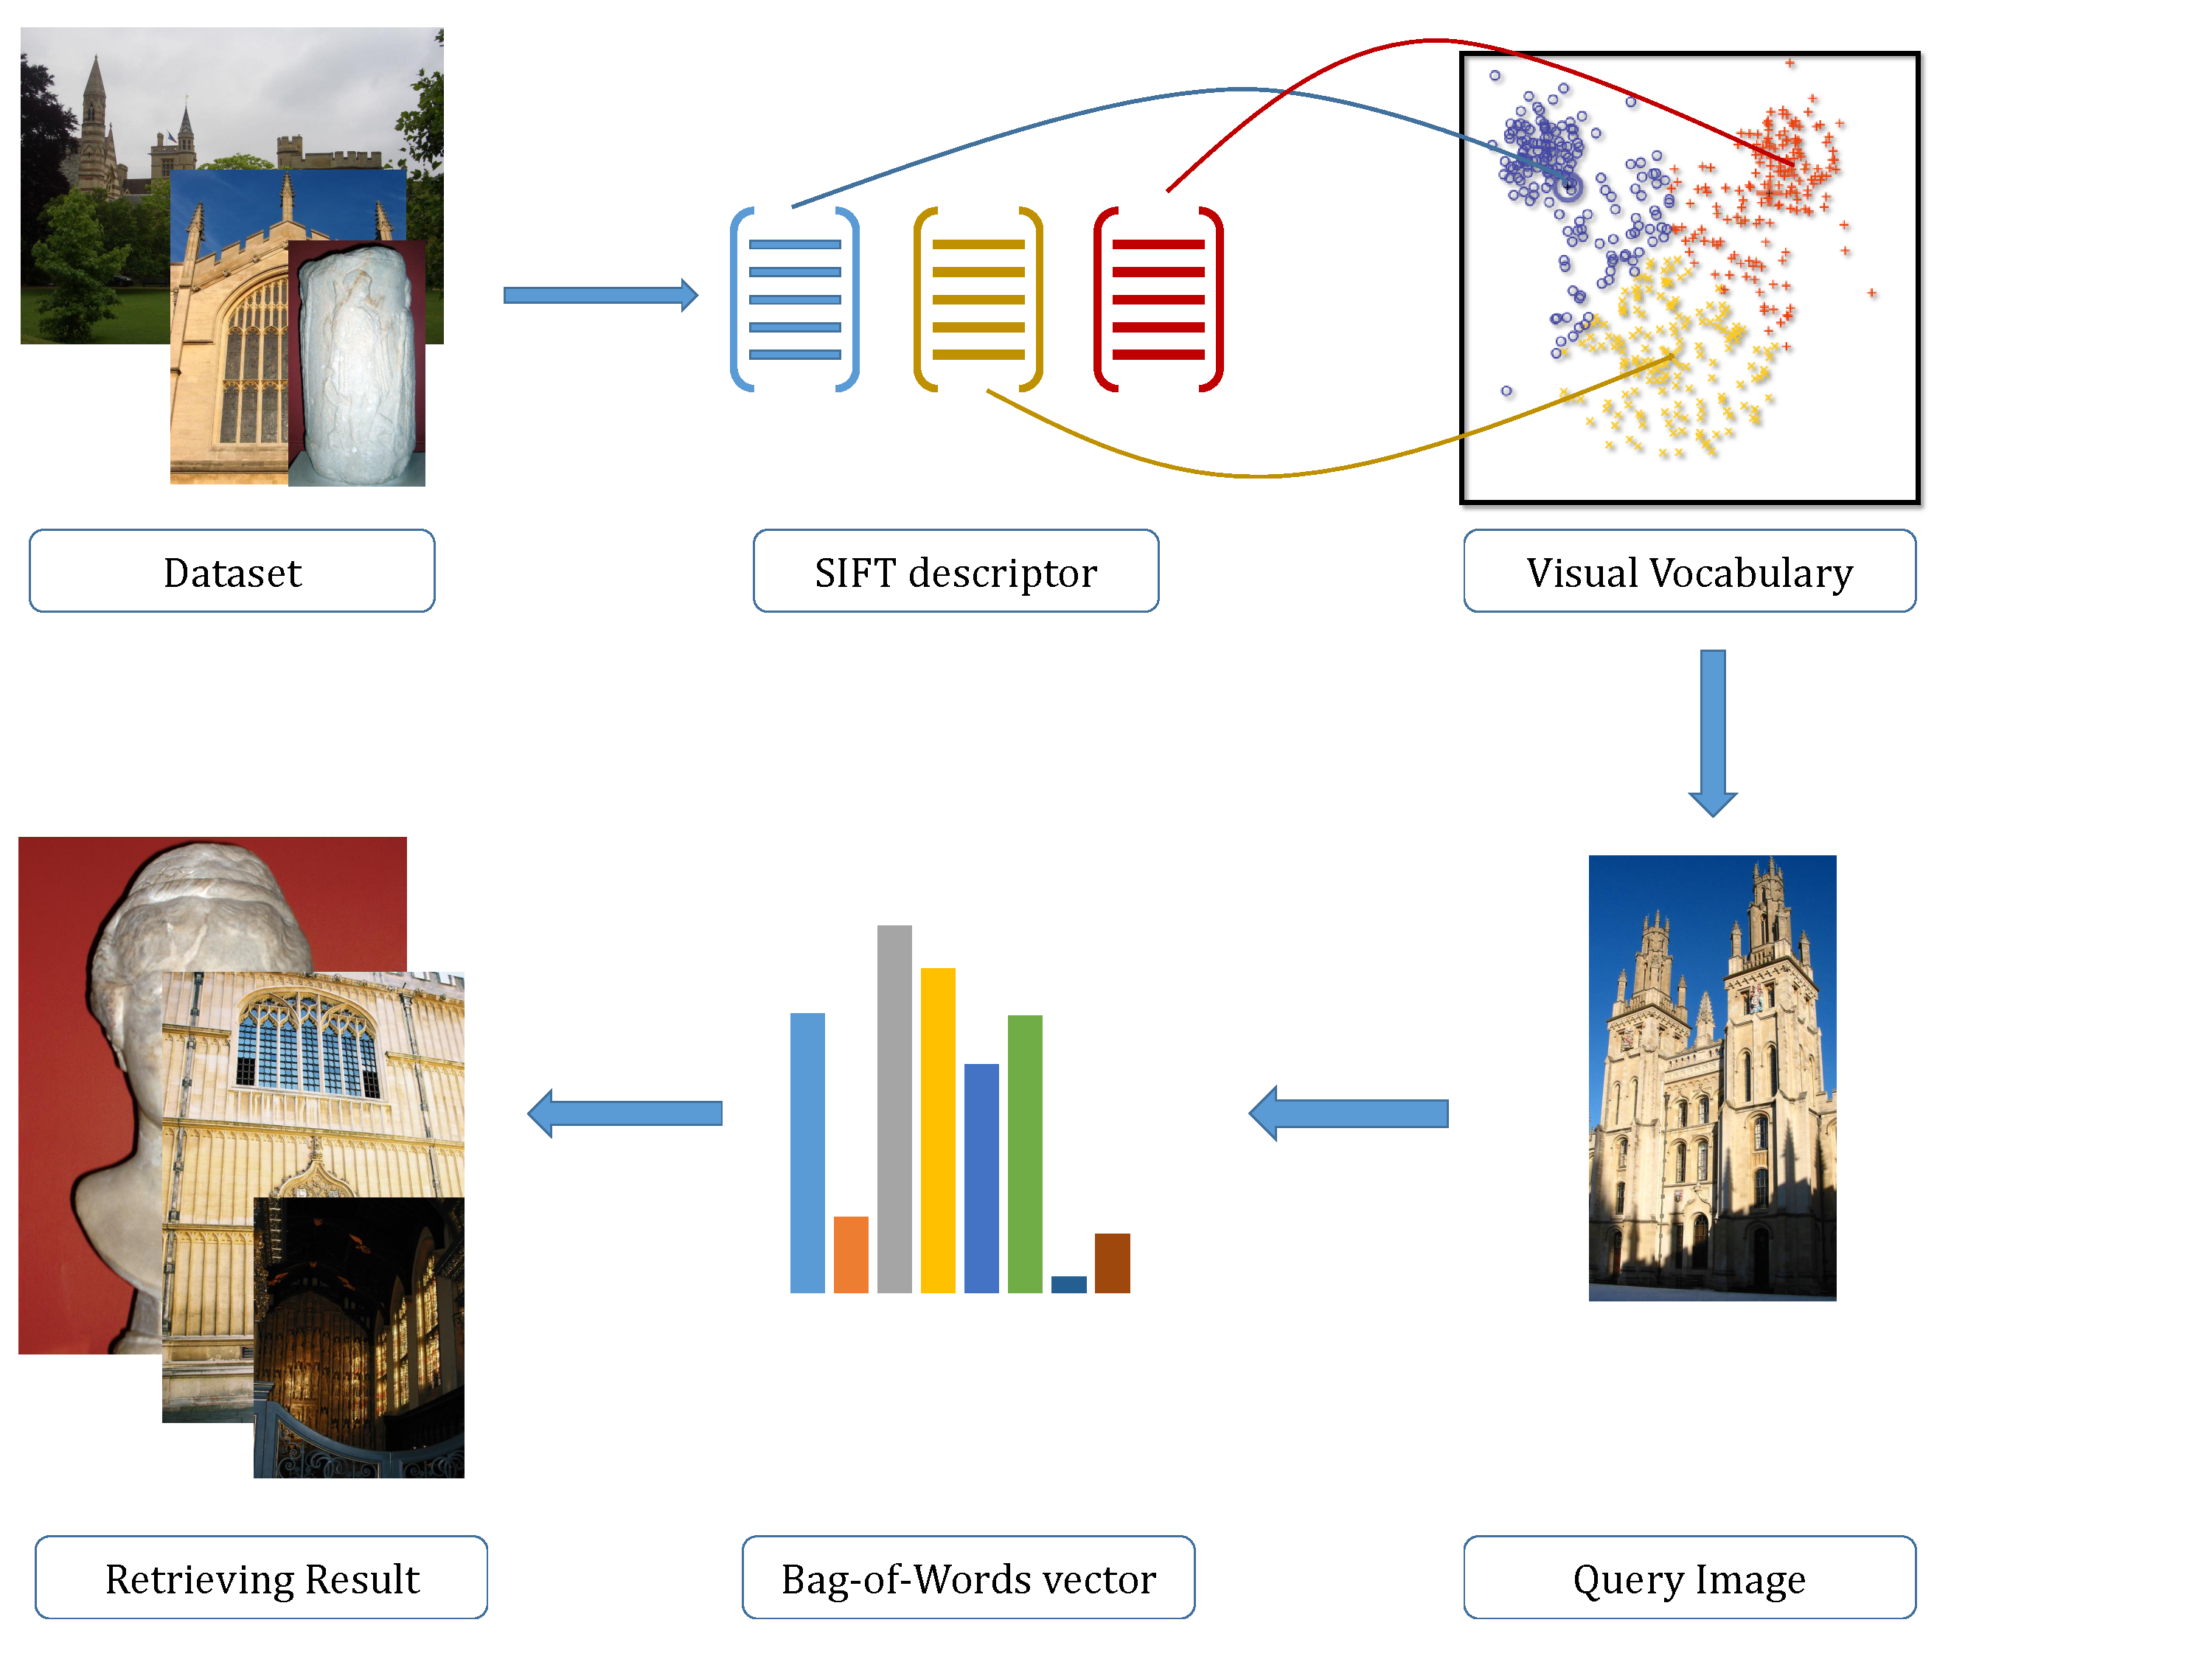
\includegraphics[width=3.0in]{process.pdf}
    \caption{Diagram of Bag-of-words model}
    \label{fig:bow_model}
\end{figure}

\subsubsection{Dictionary Building} \label{section:dictionary_building}

Generating the dictionary of visual words for such a huge amount descriptors is a big challenge. In order to overcome this obstacle, the authors use the approximate k-means (AKM) instead of the traditional exact k-means (KM). AKM is proposed by Philbin et al. \cite{2}, which reduce the majority amount of time taken by exact nearest neighbors computation by using an approximate method instead. Also, in \cite{2}, Philbin et al. shows that using 1M dictionary size would have the best performance on the Oxford Building 5K Dataset \cite{oxbuilding}.

\subsubsection{Quantization} \label{section:quantization}

Subsequently, each 128-dimension SIFT descriptor is reduced to a 3-dimension vectors of their 3 nearest visual words in the dictionary. Each of these 3 nearest cluster is assigned with weights calculated with the formula proposed by Sivic et al. \cite{7}, $weight = \exp(-\frac{d^2}{2\delta^2})$, where $d$ is the distance from the cluster center to the descriptor point and $\delta^2$ is chosen to be 6250. Then, by adding all these weights to their corresponding bins, we will have the BoW representation of an image.

\subsubsection{tf-idf Weighting Scheme} \label{section:tfidf_weighting}

As mentioned in section \ref{section:background_relatedworks}, tf-idf is a popular weighting scheme that is used by almost any BoW model. In this section, the authors will show how this scheme is applied to our system.

For a term $t_{i}$ in a particular document $d_{j}$, its term frequency $tf_{i, j}$ is defined as follow:

\begin{equation} 
        tf_{i, j} = \frac{n_{i, j}}{\sum\limits_{k} n_{k, j}}
\end{equation}
Where $n_{i, j}$ is the number of occurrences of the considered term $t_{i}$ in the document $d_{j}$. The denominator is the sum of the number of occurrences of all the terms in document $d_{j}$.

The inverse document frequency $idf_{i}$ of a term $t_{i}$ is computed by the following formula:

\begin{equation}
        idf_{i} = \log{\frac{\left|D\right|}{\left|\{j: t_{i} \in d_{j}\}\right|}}
\end{equation}
Where, $\left|D\right|$ is the total number of documents in the corpus, $\left|\{j: t_{i} \in d_{j}\}\right|$ is the number of documents where the term $t_{i}$ appears, i.e. $n_{i, j} \ne 0$

The tf-idf weight of a term $t_{i}$ in a document $d_{j}$ is then calculated as the product of tf and idf:

\begin{equation}
{tfidf}_{i, j} = tf{i, j} \times idf_{i}
\end{equation}

The tf-idf weight is then used to compute the similarity score between an image $d_{i}$ and a query $q$:

\begin{equation}
s_{d_{i}, q} = \vec{{tfidf}_{i}} \cdot \vec{{tfidf}_{q}} = \sum\limits_{j = 1}^{\left|T\right|} {tfidf}_{i, j} \times {tfidf}_{q, j}
\end{equation} 

Finally, by sorting the list of images corresponding to their similarity score with a query, we achieve the raw ranked list of this query which is then used for the Spatial Rerank step.

\subsubsection{Spatial Rerank} \label{section:spatial_rerank}

So far, we have always consider an image as a document of visual words, which means that we totally ignore the spatial structure of the features. Thus, we now incorporate the spatial constraints to the top ranked result and rerank them. The spatial verification process evaluate a geometry transformation based on features coordinates of a image and the query. The target images are then reranked using the sum of the spatial verified visual words' idf. A common approach is to use RANSAC \cite{Fischler1981}, i.e. generating different transformation hypotheses and choose the hypothese which has the largest number of ``inliers''. In our system, we perform spatial rerank on the top 800 retrieved result of the dataset, which is showed to obtain the best accuracy by Philbin et al. \cite{2}.
